%
% CRDT
%
Ein \gls{CRDT} ist eine spezielle Datenstruktur die in verteilten Systemen auf mehreren Geräten repliziert werden kann. Jede Operation wird an alle Replikate gesendet. Jedes Replikat wendet alle ankommenden Aktualisierungen an und ein Algorithmus löst alle konfliktbehafteten Aktualisierungen auf, wodurch sichergestellt ist, dass Konflikte gar nicht erst auftreten~\cite{crdt_shapiro}. Eine Synchronisation ist nicht notwendig, da die Aktualisierung sofort ausgeführt wird ~\cite{crdt_shapiro2}.\\\\
%
Es gibt zwei Konzepte bei Replikationsmodellen mit \glspl{CRDT}: den zustandsbasierten und den operationsbasierten Ansatz.
%In seinem Vortrag beschreibt Marc Shapiro die Funktionsweisen beider Ansätze und geht auf die Unterschiede, Vor- und Nachteile ein.
%Bei operationsbasierten \glspl{CRDT} muss sichergestellt werden, dass die Operationen nicht verloren gehen oder dupliziert werden wenn sie zu den anderen Replikaten übertragen werden.
%Zustandsbasierte \glspl{CRDT} haben den Nachteil, dass der gesamte Zustand, statt nur der Operation und die sich ändernden Abschnitte, zu den anderen Replikaten übertragen werden muss.
%
\subsub{Zustandbasierter Ansatz}
Wenn ein Replikat eine Aktualisierung von einem Client empfängt, wird es zuerst auf den lokalen Status angewandt.
Dann sendet es etappenweise eine Kopie des eigenen, aktualisierten Status an andere Replikate im System.
Wenn ein Replikat den Status eines anderen Replikats empfängt, führt es mit einer \tt{merge} Funktion den empfangenen Status mit dem lokalen zusammen.
Entsprechend sendet dieses Replikat gelegentlich auch seinen Status an ein anderes Replikat, sodass jede Aktualisierung schließlich alle Replikate im System erreicht ~\cite{crdt_shapiro2}.
Die folgende Abbildung stellt eine zustandsbasierte Replikation mit drei Geräten dar.
%
\begin{figure}[H]
  \centering
  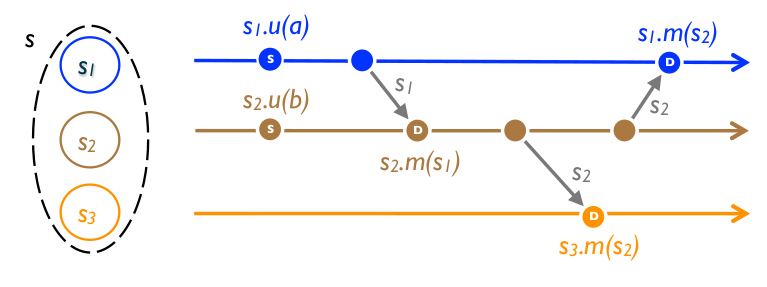
\includegraphics[width=0.8\textwidth]{crdt-state}
  \grayRule
  \caption[Replikation von zustandsbasierten \glspl{CRDT}]{Replikation von zustandsbasierten \glspl{CRDT}, Quelle: ~\cite{crdt_shapiro2}}
  \label{fig:crdt-state}
\end{figure}
%
Die drei Kreise auf der linken Seite repräsentieren drei identische Datensätze auf drei Geräten. Die Datensätze \it{S1} und \it{S2} werden zeitgleich mit unterschiedlichem Kontent aktualisiert.
Kurz darauf, weiter rechts im Bild, sendet \it{S1} seinen neuen Status an \it{S2}.
\it{S2} führt die beiden Status, den von \it{S1} empfangenen und den eigenen, aktualisierten, in der \tt{merge} Funktion $m$ zusammen.
Dann schickt es den eigenen, neuen Status an \it{S3} und \it{S1}, welche ebenfalls den empfangenen mit dem eigenen Status zusammenführen. Beide Aktualisierungen haben nun alle Geräte erreicht und alle Daten sind identisch.\\\\
%
Damit die Replikation konfliktfrei funktioniert müssen einige Voraussetzungen erfüllt sein.
Der Status, den ein \gls{CRDT} hat muss ein Semi--Gitter, also eine geordnete Menge abbilden.
Die Aktualisierungen müssen zunehmend sein, ein Status kann beispielsweise eine Zahl sein und die Aktualisierung ist die Operation die sie inkrementiert.
Die \tt{merge} Funktion muss die kleinste obere Grenze der letzten Aktualisierung berechnen.
Nur wenn ein Objekt diese Eigenschaften erfüllt, ist es dem \gls{CRDT} zugehörig ~\cite{crdt_shapiro2}
%
%
%
\subsub{Operationsbasierter Ansatz}
Wenn ein Replikat eine Aktualisierung von einem Client empfängt, wird es ebenfalls zuerst auf den lokalen Status angewandt.
Im Gegensatz zum zustandsbasiertem Ansatz wird nicht der gesamte Status des Replikats gesendet, sondern nur der Aktualisierungsvorgang.
Ein weiterer Unterschied ist das Fehlen der \tt{merge} Funktion. Statt ihrer gibt es im operationsbasierten Ansatz zwei \tt{update} Methoden: eine vorbereitende Aktualisierungsfunktionen und eine ausführende. Erstere wird auf dem Replikat angewandt, umgehend gefolgt von der zweiten.
Über ein Kommunikationsprotokoll wird die Aktualisierung an alle anderen Replikas asynchron versendet.
Über das Protokoll wird sichergestellt, dass die Nachricht nur einmal überliefert wird.
Die restlichen Replikas wenden die Operation mit der ausführenden Aktualisierungsmethode auf sich an~\cite{crdt_shapiro2}.
Die folgende Abbildung stellt eine operationsbasierte Replikation mit drei Geräten dar.
%
\begin{figure}[H]
  \centering
  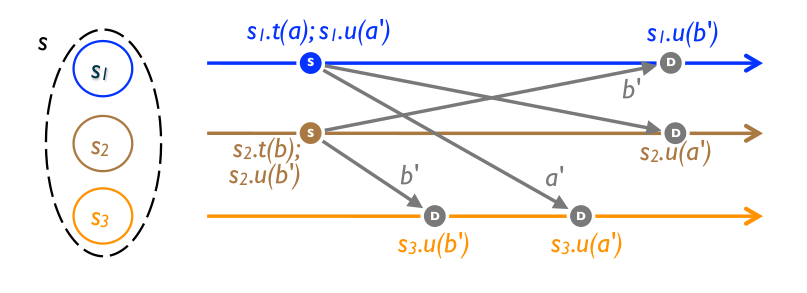
\includegraphics[width=0.8\textwidth]{crdt-op}
  \grayRule
  \caption[Replikation von Operationsbasierten \gls{CRDT}]{Replikation von Operationsbasierten \glspl{CRDT}, Quelle: ~\cite{crdt_shapiro2}}
  \label{fig:crdt-op}
\end{figure}
%
Die drei Kreise auf der linken Seite repräsentieren drei identische Datensätze auf drei Geräten. Die Datensätze \it{S1} und \it{S2} werden zeitgleich mit unterschiedlichem Kontent aktualisiert.
Sowohl \it{S1} also auch \it{S2} wenden die vorbereitende Aktualisierungsmethode $t$ auf sich an.
Dann, mit dessen Ergebnis, die ausführende $u$.
Sofort senden beide Replikas die Aktualisierung an alle anderen, welche ebenfalls die ausführende Aktualisierungsmethode $u$ auf sich anwenden.\\\\
Die Voraussetzung für eine konfliktfreie Replikation sind hier kommuntative Aktualisierungen.
%Wenn $s$ der Status ist und $u$ die Aktualisierungsmethode, muss $s \bullet u \bullet u' \equiv s \bullet u' \bullet u$ gelten.
Nur so spielt die Reihenfolge in der die Aktualisierungen bei den Replikaten ankommen keine Rolle -- das Ergebnis ist dasselbe ~\cite{crdt_shapiro2}.\\\\
Umgesetzte \glspl{CRDT} sind zum Beispiel Counter, ein Datenobjekt das zum Zählen verwendet wird. Es gibt einen, der nur hochzählen kann und eine andere Variante die auch die Subtraktion unterstützt.
Weitere \glspl{CRDT} sind Sets, eine Listenrepräsentation ohne Duplikate. Auch hier gibt es eine Variante mit der nur Daten hinzugefügt werden können und eine die auch das Entfernen der Daten erlaubt ~\cite{crdt_shapiro}.
%
%CRDTs befassen sich mit einem interessanten und grundlegendem Problem in verteilten Systemen, haben jedoch eine wichtige Einschränkung:
%"Da ein CRDT konstruktionsbedingt keinen Konsens verwendet, hat der Ansatz starke Einschränkungen; Dennoch sind einige interessante und nicht-triviale CRDTs bekannt" ~\cite{crdt_shapiro2}.
%Die Einschränkung ist, dass die CRDT-Adresse nur einen Teil des Problemraums betrifft, da nicht alle möglichen Aktualisierungsoperationen kommutativ sind und daher nicht alle Probleme in CRDTs umgewandelt werden können.
%
%Alas, everything in programming is trade-offs, so what do we trade for being able to have conflict-free data structures? Well, they are specialised data structures, like sets and counters, and not generic object representations like JSON, so we’ll have to buy into a whole world of these specialised data structures, and maybe we have hard time mapping our application objects to them. 